%A compiler en XELATEX sinon pas d'arbre de proba
\documentclass[french]{book}
\usepackage{teach}
\usepackage{verbatim}
\usepackage[french]{babel}
%%% Couleurs
\redefinecolor{thm}{title}{bgcolor}{alizarin}
\redefinecolor{prop}{title}{bgcolor}{meatbrown}
\redefinecolor{defn}{title}{bgcolor}{olivine}
\definecolor{alizarin}{rgb}{0.82, 0.1, 0.26}
\definecolor{meatbrown}{rgb}{0.9, 0.72, 0.23}
\definecolor{olivine}{rgb}{0.6, 0.73, 0.45}
\usepackage{color}
%%%%%%Les symboles
\usepackage{amsmath}
\usepackage{amssymb}
\usepackage{amsfonts}
\usepackage{amsthm}
\usepackage{mwe}
\usepackage{yhmath} 
\usepackage{eurosym}
%%% Ensemble de nombre
\newcommand{\R}{\mathbb{R}}
%\newcommand{\C}{\mathds {C}}
\newcommand{\N}{\mathbb{N}}
\newcommand{\Z}{\mathbb{Z}}
\newcommand{\Q}{\mathbb{Q}}
\newcommand{\D}{\mathbb{D}}
%%% Tableau
\usepackage{array}
\usepackage{multicol}
\setlength{\multicolsep}{3pt}
%%% Figures
\usepackage{tikz}
\usepackage{graphicx}
\graphicspath{{Figures/}}
%\usepackage{pstricks,pst-plot,pst-text,pst-tree,pst-eucl}
%%%Affichage
\newcommand{\ds}{\displaystyle}
\renewcommand{\arraystretch}{1.2} 
\newcolumntype{C}[1]{>{\centering\arraybackslash}p{#1cm}}
%%% Lecon creuse/pleine
\usepackage{dashundergaps}
\TeacherModeOff
%\TeacherModeOn
%%% Macro
\newcommand{\V}{\overrightarrow}
\newcommand{\Rep}{(O;\V{i};\V{j})}
\newcommand{\Syst}[2]{\left\{\begin{array}{lcccc} #1 \\ #2 \end{array}\right.}
\begin{document}

\chapter{Statistiques à deux variables}

\section{Position du problème, vocabulaire}
\emph{Le problème qui se pose dans les séries statistiques à deux variables est principalement celui du lien qui existe ou non entre chacune des variables. 
Par soucis de clarté, ce cours est élaboré à partir de l'exemple suivant :}



\begin{exemple}
Le tableau suivant donne l'évolution du nombre d'adhérents d'un club de rugby de $2001$ à $2006$.
\begin{center}
   \begin{tabular}{|c|*{6}{C{1}|}}
      \hline
      Année & $2001$ & $2002$ & $2003$ & $2004$ & $2005$ & $2006$ \\
      \hline
      Rang $x_{i}$ & $1$ & $2$ & $3$ & $4$ & $5$ & $6$ \\
      \hline
      Nombre d'adhérents $y_{i}$ & $70$ & $90$ & $115$ & $140$ & $170$ & $220$ \\
      \hline
   \end{tabular}
\end{center}
Le but est d'étudier cette série statistique à deux variables (le rang et le nombre d'adhérents) afin de prévoir l'évolution du nombre d'adhérents pour les années suivantes.
\end{exemple}

%%%   I.1   %%%%%%%%%%%%%%%%%%%%%%%%%%%%%%%%%%%%%%%%%%%
\subsection{Nuage de points}

La première étape consiste à réaliser un graphique qui traduise les deux séries statistiques ci-dessus.

\begin{defn}
   Soit $X$ et $Y$ deux variables statistiques numériques observées sur $n$ individus.\\
   Dans un repère orthogonal $\Rep$, l'ensemble des $n$ points de coordonnées $(x_i,y_i)$ forme le \underline{nuage de points} associé à cette série statistique.
\end{defn}

Dans notre exemple, si on place le rang en abscisses, et le nombre d'adhérents en ordonnées, on peut représenter par un point chaque valeur. On obtient ainsi une succession de points, dont les coordonnées sont $(1;70)$, $(2;90)$, ... $(6;220)$, forment un \underline{nuage de points}.



\begin{exemple}
   Dans le plan muni d'un repère orthogonal d'unités graphiques : $1,5$~cm pour une année sur l'axe des abscisses et $1$~cm pour $20$~adhérents sur l'axe des ordonnées, représenter le nuage de points associé à la série $(x_{i};y_{i})$.
\end{exemple}

\begin{color}{blue}
   \begin{multicols}{2}
   T.I.
   \begin{itemize}
      \item[$\bullet$] Touche \fbox{STAT}
      \item[$\bullet$] Menu \fbox{EDIT}
      \item[$\bullet$] Entrer les valeurs $x_i$ dans $L_1$
      \item[$\bullet$] Entrer les valeurs $y_i$ dans $L_2$
      \item[$\bullet$] Règler les valeurs du repère avec la touche \fbox{WINDOWS}
      \item[$\bullet$] Appuyer sur la touche \fbox{TRACE}
   \end{itemize}
   Casio
   \begin{itemize}
      \item[$\bullet$] Menu \fbox{STAT}
      \item[$\bullet$] Entrer les valeurs $x_i$ dans $List 1$
      \item[$\bullet$] Entrer les valeurs $y_i$ dans $List 2$
      \item[$\bullet$] Choisir \fbox{GRPH}
      \item[$\bullet$] Règler les paramètres avec \fbox{SET}
      \item[$\bullet$] Choisir \fbox{GPH1}
   \end{itemize}
   \end{multicols}
\end{color}
\newpage 
\begin{center}
\includegraphics[scale=1]{stat.1}
\end{center}

\subsection{Le problème de l'ajustement}

\begin{rem}
Le nuage de points associé à une série statistique à deux variables donne donc immédiatement des informations de nature qualitatives. Pour en tirer des informations plus quantitatives, il nous faut poser le problème de l'ajustement. Le tracé met en évidence la possibilité de "reconnaître" graphiquement la possibilité d'une relation fonctionnelle entre les deux grandeurs observées (ici rang et nombre d'adhérent).
Le problème de l'établissement d'une relation fonctionnelle entre les deux séries est le \underline{problème de l'ajustement}. 
\end{rem}

\vfill

%%%   I.3   %%%%%%%%%%%%%%%%%%%%%%%%%%%%%%%%%%%%%%%%%%%
\subsection{Point moyen}

\begin{defn}
   Soit une série statistique à deux variables, $X$ et $Y$, dont les valeurs sont des couples $(x_i;y_i)$.\\
   On appelle \underline{point moyen} de la série le point $G$ de coordonnées
   \begin{itemize}
      \item[$\bullet$] $x_G=\dfrac{x_1+x_2+ \dots + x_n}{n}=\bar{x}$.
      \item[$\bullet$] $y_G=\dfrac{y_1+y_2+ \dots + y_n}{n}=\bar{y}$.
   \end{itemize}
\end{defn}

\begin{exemple}
   Déterminer les coordonnées des points moyens suivants :
   \begin{itemize}
      \item[$\bullet$] $G_1$ des années allant de $2001$ à $2003$,
      \item[$\bullet$] $G_2$ des années allant de $2004$ à $2006$,
      \item[$\bullet$] $G$, point moyen du nuage de points tout entier.
   \end{itemize}
\end{exemple}

Calcul des coordonnées de $G_1$ : $\Syst{x_{G_1} & = & \frac{1+2+3}{3} & = & 2}{y_{G_1} & = & \frac{70+90+115}{3} & = & 91,7}$ \qquad donc, ~ \fbox{$G_1(~2~;~91,7~)$}.

Calcul des coordonnées de $G_2$ : $\Syst{x_{G_2} & = & \frac{4+5+6}{3} & = & 5}{y_{G_2} & = & \frac{140+170+220}{3} & = & 176,7}$ \qquad donc, ~ \fbox{$G_2(~5~;~176,7~)$}.

Calcul des coordonnées de $G$ : $\Syst{x_G & = & \frac{1+2+3+4+5+6}{6} & = & 3,5}{y_G & = & \frac{70+90+115+140+170+220}{3} & = & 134,2}$ \qquad donc, ~ \fbox{$G(~3,5~;~134,2~)$}.


%%%%%%%%%%%%%%%%%%%%%%%%%%%%%%%%%%%%%%%%%%%%%%%%%%%%%
%%%   II   %%%%%%%%%%%%%%%%%%%%%%%%%%%%%%%%%%%%%%%%%%
%%%%%%%%%%%%%%%%%%%%%%%%%%%%%%%%%%%%%%%%%%%%%%%%%%%%%
\section{Ajustements}


%%%   II.1   %%%%%%%%%%%%%%%%%%%%%%%%%%%%%%%%%%%%%%%%%%%
\subsection{Ajustement à la règle}

On se propose, à partir des résultats obtenus, de faire des prévisions pour les années à venir. \\
Un moyen d'y parvenir est de tracer au juger une droite $\mathcal{D}$ passant le plus près possible des points du nuage et d'en trouver l'équation du type $y=ax+b$.


%%%   II.2   %%%%%%%%%%%%%%%%%%%%%%%%%%%%%%%%%%%%%%%%%%
\subsection{Méthode de Mayer}

Cet ajustement consiste à déterminer la droite passant par deux points moyens du nuage de point.


\begin{exemple}
   Déterminer l'équation de la droite $\mathcal{D}_1$ qui passe par les points moyens $G_1$ et $G_2$ et la tracer sur le graphique précédent.
\end{exemple}

La droite $\mathcal{D}_1$ n'est pas parallèle à l'axe des ordonnées, elle a donc pour équation $y=ax+b$ avec : \\
$a=\dfrac{y_{G_2}-y_{G_1}}{x_{G_2}-x_{G_2}}=\frac{176,7-91,7}{5-2}=28,3$.

De plus, elle passe par le point $G_1(~2~;~91,7~)$ d'où : \\
$y_{G_1}=ax_{G_1}+b \quad \Rightarrow \quad 91,7=28,3\times 2+b \quad \Rightarrow \quad b=35,1$.

Conclusion : \fbox{$\mathcal{D}_1 : y=28,3x+35,1$}.

Pour tracer $\mathcal{D}_1$, il suffit de placer $G_1$ et $G_2$ puis de tracer la droite qui les relie.


\begin{center}
\includegraphics[scale=1]{stat.2}
\end{center}

%%%   II.3   %%%%%%%%%%%%%%%%%%%%%%%%%%%%%%%%%%%%%%%%%%
\subsection{Méthode des moindres carrés}

Il s'agit d'obtenir une droite qui minimise la distance entre la droite et les points situés de part et d'autre d'elle-même. \\
Pour réaliser ceci, on cherche à minimiser la somme des distances des points à la droite au carré, ce qui permet de ne pas tenir compte du signe des écarts.

On considère une série statistique à deux variables représentée par un
nuage justifiant un ajustement affine.



\begin{defn}
   Dans le plan muni d'un repère orthonormal, on considère un nuage de $n$ points $(M_i)$ de coordonnées $(x_i;y_i)$ et $n$ points $Q_i$ de coordonnées $(x_i;ax_i+b)$ tous aligné sur la droite d'équation $y=ax+b$.\\
   La droite $\mathcal{D}$ d'équation $y=ax+b$ est appelée \underline{droite de régression} de $y$ en $x$ de la série statistique si et seulement si la quantité suivante est minimale :
   $$\sum_{i=1}^n~(M_iQ_i)^2=\sum_{i=1}^n [y_i-(ax_i+b)]^2$$
\end{defn}

\begin{exemple}
Représentation graphique d'une droite de régression de $y$ en $x$ pour un nuage de $6$ points.
\begin{center}
\includegraphics[scale=1]{stat.3}
\end{center}
\end{exemple}
\vspace*{2cm}

\begin{rem}
   Il serait tout aussi judicieux de s'intéresser à la droite $\mathcal{D}'$ qui minimise la quantité $\displaystyle{\sum_{i=1}^n [x_i-(ay_i+b)]^2}$. \\
   Cette droite est appelée droite de régression de $x$ en $y$.
\end{rem}

\newpage


\begin{defn}
   On appelle \underline{covariance} de la série statistique double de variables $x$ et $y$ le nombre réel
$$cov(x,y)=\sigma_{xy}=\frac1n\sum_{i=1}^n (x_i - \bar x) (y_i - \bar y).$$
\end{defn}

\begin{prop}
Pour les calculs, on pourra aussi utiliser la formule de König:
$$\sigma_{xy}=\frac1n(\sum_{i=1}^n x_i y_i)-\bar x\bar y.$$
\end{prop}

\begin{rem}
   On a : \quad $cov(x,x)=\sigma_{x^2}=V(x)=[\sigma(x)]^2$.
\end{rem}



\begin{prop}
   La droite de régression $D$ de $y$ en $x$ a pour équation $y=ax+b$ où 
   
  %$$\Syst{a=\dfrac{\sigma_{xy}}{\sigma_{x}^2}}{b\rm{~~vérifie~~}\bar y=a\bar x+b.}$$
  
  $$\Syst{a=\dfrac{\sigma_{xy}}{\sigma_{x}^2}}{b \; \text{vérifie} \; \bar y = a\bar x +b}$$
\end{prop}

\begin{rem}
   Les réels $a$ et $b$ sont donnés par la calculatrice.
\end{rem}

\begin{color}{blue}
\begin{multicols}{2}
   T.I.
   \begin{itemize}
      \item[$\bullet$] Touche \fbox{STAT}
      \item[$\bullet$] Menu \fbox{CALC}
      \item[$\bullet$] Item \fbox{LinReg}
      \item[$\bullet$] LinReg $L_1,L_2$ \\
   \end{itemize}
   Casio
   \begin{itemize}
      \item[$\bullet$] Menu \fbox{STAT}
      \item[$\bullet$] Item \fbox{CALC}
      \item[$\bullet$] Règler les paramètres avec\fbox{set}
      \item[$\bullet$] Item \fbox{REG}
      \item[$\bullet$] Choisir \fbox{X}
   \end{itemize}
\end{multicols}
\end{color}



\begin{prop}
   Le point moyen $G$ du nuage appartient toujours à la droite de régression de $y$ en $x$.
\end{prop}



\begin{exemple}
Déterminer une équation de la droite d'ajustement $\mathcal{D}_2$ de $y$ en $x$ \emph{obtenue par la méthode des moindres carrés} pour la série statistique de l'exemple 1.
\end{exemple}

La calculatrice donne $\mathcal{D}_2:y=ax+b$ avec $a=29$ et $b=32,7$.

Conclusion : \fbox{$\mathcal{D}_2:y=29x+32,7$}

Pour tracer la droite $\mathcal{D}_2$, il faut choisir deux points (au moins) sur cette droite.\\
Par exemple : \quad 
\begin{tabular}{C{1}|C{1}|C{1}}
   $x$ & $0$ & $8$ \\
   \hline
   $y$ & $32,7$ & $264,7$ \\
\end{tabular}
\quad , les placer dans le repère puis tracer la droite.
\vfill

\begin{center}
\includegraphics[scale=1]{stat.4}
\end{center}

%%%   II.4   %%%%%%%%%%%%%%%%%%%%%%%%%%%%%%%%%%%%%%%%%%
\newpage
\subsection{Ajustement exponentiel}%%%%%%%%%%%%%%%%%%%%%

On remarque qu'un ajustement affine ne semble pas très approprié pour ce nuage de points à partir de $2006$, on se propose de déterminer un ajustement plus juste.



\begin{exemple}
   On pose $z=\log y$. Recopier et compléter le tableau suivant en arrondissant les valeurs de $z_{i}$ au millième. 
   \begin{center}
      \begin{tabular}{|*{7}{C{1}|}}
         \hline
         $x_{i}$ & $1$ & $2$ & $3$ & $4$ & $5$ & $6$ \\
         \hline
         $z_{i}$ & $1,845$ & $1,954$ & $2,060$ & $2,146$ & $2,230$ & $2,342$ \\
         \hline
      \end{tabular}
   \end{center}
\end{exemple}

%Il suffit de calculer $\ln y_i$ pour chaque caleur de $i$ :
%\begin{center}
%   \begin{tabular}{|*{7}{C{1}|}}
%      \hline
%      $x_{i}$ & $1$ & $2$ & $3$ & $4$ & $5$ & $6$ \\
%      \hline
%      $z_{i}$ & $4,248$ & $4,500$ & $4,745$ & $4,942$ & $5,136$ & $5,394$ \\
%      \hline
%   \end{tabular}
%\end{center}

On peut déterminer les éléments de ce tableau grâce à la calculatrice :

\begin{color}{blue}
\begin{multicols}{2}
   T.I.
   \begin{itemize}
      \item[$\bullet$] Touche \fbox{STAT}
      \item[$\bullet$] Menu \fbox{EDIT}
      \item[$\bullet$] Se placer dans \fbox{$L_3$}
      \item[$\bullet$] Entrer la formule "$=\log L_2$"
   \end{itemize}
   Casio
   \begin{itemize}
      \item[$\bullet$] Touche \fbox{STAT}
      \item[$\bullet$] Menu \fbox{EDIT}
      \item[$\bullet$] Se placer sur \fbox{$List3$}
      \item[$\bullet$] Entrer la formule "$\log List2$"
   \end{itemize}
\end{multicols}
\end{color}




\begin{exemple}
   Déterminer une équation de la droite d'ajustement $\mathcal{D}_3$ de $z$ en $x$ obtenue par la méthode des moindres carrés.  
\end{exemple}

La manipulation à la calculatrice est la même que précédemment, en oubliant pas de changer les paramètres.

La calculatrice donne $\mathcal{D}_3:z=ax+b$ avec $a=0,224$ et $b=4,045$.

Conclusion : \fbox{$\mathcal{D}_3:z=0,0971x+1,75627$}.



\begin{exemple}
   Dans ce cas, en déduire la relation qui lie $y$ à $x$ puis tracer la courbe représentative de la fonction $y=f(x)$.
\end{exemple}

On a $\Syst{z & = & 0,0971x+1,75627}{z & = & \log y}$ \quad donc : \quad $\log y=0,0971x+1,75627$

On compose par la fonction exponentielle :
\begin{tabular}[t]{ccl}
   $10^{\ln y} $& $=$ &$ 10^{0,0971x+1,75627}$ \\
    &$ = $&$ (10^{0,0971})^x\times 10^{1,75627}$ \\
    &$ =$ & $(1,251)^x\times 57,052$ \\
\end{tabular}

Conclusion : \fbox{$y=57,052\times1,251^x$}.

Pour tracer la courbe, il suffit de placer des points, par exemple grâce au tableau de valeurs de la calculatrice.

\begin{center}
\includegraphics[scale=1]{stat.5}
\end{center}
%%%   II.5   %%%%%%%%%%%%%%%%%%%%%%%%%%%%%%%%%%%%%%%%%%
\newpage
\section{Comparaisons des ajustements}

Grâce aux trois derniers ajustements, on peut évaluer ce qui se passera plus tard, comparons les :


\begin{exemple}
   En supposant que les ajustements restent valables pour les années suivantes, donner une estimation du nombre d'adhérents en $2007$ suivant les trois méthodes.
\end{exemple}

Dans tous les cas, il faut calculer $y$ lorsque $x$ correspond à l'année $2007$, c'est à dire au rang $7$.

\begin{itemize}
   \item[$\bullet$] Méthode de Mayer : $y=28,3\times7+35,1=233,2$ soit environ \fbox{$233$ adhérents}.
   \item[$\bullet$] Ajustement affine : $y=29\times 7+32,7=235,7$ soit environ \fbox{$236$ adhérents}.
   \item[$\bullet$] Ajustement exponentiel : $y=57,112\times1,024^7=273,9$ soit environ \fbox{$274$ adhérents}.
\end{itemize}



\begin{exemple}
   En $2007$, il y a eu $280$ adhérents. Lequel des trois ajustements semble le plus pertinent ?
\end{exemple}

Le troisième ajustement semble le plus pertinent puisqu'il se rapporche le plus de la réalité.

%%%%%%%%%%%%%%%%%%%%%%%%%%%%%%%%%%%%%%%%%%%%%%%%%%%%%
%%%   III   %%%%%%%%%%%%%%%%%%%%%%%%%%%%%%%%%%%%%%%%%
%%%%%%%%%%%%%%%%%%%%%%%%%%%%%%%%%%%%%%%%%%%%%%%%%%%%%
\subsection{Coefficient de corrélation linéaire}

\begin{defn}
   Le \underline{coefficient de corrélation linéaire} d'une série statistique de variables $x$ et $y$ est le nombre $r$ défini par :
   $$r=\frac{\sigma_{xy}}{\sigma(x)\times\sigma(y)}.$$
\end{defn}

Ce coefficient sert à mesurer la qualité d'un ajustement affine.


\textbf{Interprétation graphique :} \\
Plus le coefficient de régression linéaire est proche de $1$ en valeur absolue, meilleur est l'ajustement linéaire. \\
Lorque $r=\pm1$, la droite de régression passe par tous les points du nuage, qui sont donc alignés.


\begin{exemple}
   Déterminer le coefficient de corrélation linéaire dans le cas de l'ajustement affine (entre $x$ et $y$), puis exponentiel (entre $x$ et $z$). Quel est l'ajustemet le plus juste ?
\end{exemple}

Grâce à la calculatrice, on trouve successivement $r_2=0,987$ puis $r_3=0,999$. \\
Ce qui est conforme à ce que nous avions déduit précédemment, à savoir que l'ajustement exponentiel est plus fiable pour ce cas.



\begin{prop}
   Le  coefficient de corrélation linéaire $r$ vérifie $-1\leq r\leq 1$.
\end{prop}


\newpage
\section{Exercices}
%%Pascal Brachet
\begin{exocor}
Calculer les coordonnées du point moyen de la série suivante :\\
\begin{center}
\begin{tabular}{|c|c|c|c|c|c|}
\hline $ x_{i} $ & 200 & 205 & 208 & 211 & 215 \\ 
\hline $ y_{i} $ & 5200 & 5400 & 5600 & 5900 & 6400 \\ 
\hline 
\end{tabular}
\end{center}
\end{exocor}

\begin{exocor}
Déterminer $ x $ et $ y $ pour que le point moyen de la série soit de coordonnées $ (7,5 \: ; \: 12,6) $.\\
\begin{center}
\begin{tabular}{|c|c|c|c|c|c|}
\hline $ x_{i} $ & 8,2 & 7,4 & $ x $ & 6,1 & 9 \\ 
\hline $ y_{i} $ & 15 & 12,1 & 16,3 & $ y $ & 12 \\ 
\hline 
\end{tabular}
\end{center}
\end{exocor}

\begin{exocor}
On considère la série statistique double ci-dessous.\\
\begin{center}
\begin{tabular}{|c|c|c|c|c|c|c|}
\hline $ x_{i} $ & 1 & 3 & 4 & 6 & 7 & 8 \\ 
\hline $ y_{i} $ & 11,1 & 13 & 14,5 & 16 & 16,9 & 19 \\ 
\hline 
\end{tabular}
\end{center}
\begin{enumerate}
\item Représenter le nuage de points $ M_{i}(x_{i},y_{i}) $ dans un repère orthonormé.
\item Calculer les coordonnées du point moyen et placer ce point dans le repère.
\item Donner une équation de la droite de régression de $ y $ en $ x $ obtenue par la méthode des moindres carrés et tracer cette droite dans le repère. \textit{($ a $ et $ b $ seront arrondis à $0,01$ près)}
\end{enumerate}
\end{exocor}

\begin{exocor}
Le tableau suivant donne la moyenne $ y $ des maxima de tension artérielle en fonction de l'âge $ x $.\vspace*{0.1cm}\\
\begin{center}
\begin{tabular}{|c|c|c|c|c|c|c|c|}
\hline âge $ x_{i} $ & 36 & 42 & 48 & 54 & 60 & 66 & 70 \\ 
\hline tension $ y_{i} $ & 12 & 13 & 13,6 & 14,3 & 15,4 & 15,8 & 16 \\ 
\hline 
\end{tabular}
\end{center}
\begin{enumerate}
\item Donner une équation de la droite de régression de $ y $ en $ x $ obtenue par la méthode des moindres carrés. \textit{($ a $ et $ b $ seront arrondis à $0,01$ près)}
\item Quelle serait la tension théorique d'une personne de 75 ans en utilisant le modèle de la droite des moindres carrés ? \textit{(arrondir le résultat à $0,1$ près)}
\end{enumerate}
\end{exocor}

\begin{exocor}
Le tableau suivant indique la teneur en $ \mathrm{CO_{2}} $ depuis 1850.\vspace*{-0.3cm}\\

\begin{center}
\begin{tabular}{|c|c|c|c|c|}
\hline Année & 1850 & 1900 & 1950 & 1990 \\ 
\hline Rang de l'année : $ x_{i} $ & 0 & 50 & 100 & 140 \\ 
\hline Teneur en $\mathrm{CO_{2}} $ : $ y_{i} $ & 275 & 290 & 315 & 360 \\ 
\hline $ z_{i}=\log (y_{i}-250) $ &  &  &  &  \\ 
\hline 
\end{tabular}
\end{center}

\begin{enumerate}
\item Compléter dans le tableau la ligne indiquant $ z_{i}=\log (y_{i}-250) $.
\item Donner une équation de la droite de régression de $ z $ en $ x $ obtenue par la méthode des moindres carrés. \textit{($ a $ et $ b $ seront arrondis à $0,01$ près)}
\item Selon ce modèle, quel serait le taux de $ \mathrm{CO_{2}} $ en 2050? \textit{(donner le résultat à une unité près)}
\end{enumerate}

\end{exocor}

\begin{exocor}
Le tableau suivant donne le nombre d'abonnés à un jeu en ligne. 
\begin{center}
\begin{tabular}{|c|c|c|c|c|c|}
\hline Année & 2014 & 2015 & 2016 & 2017 & 2018 \\ 
\hline Rang de l'année $ x_{i} $ & 1 & 2 & 3 & 4 & 5 \\ 
\hline Nombre d'abonnés $ y_{i} $ (en milliers) & 40 & 80 & 130 & 260 & 420 \\ 
\hline $ z_{i}=\log y_{i} $  &  &  &  &  &  \\ 
\hline 
\end{tabular}
\end{center}
\begin{enumerate}
\item Le nuage de points $ A_{i}(x_{i},y_{i}) $ est représenté ci-dessous. Un ajustement affine vous semble-t-il adapté ?\\
\begin{center}
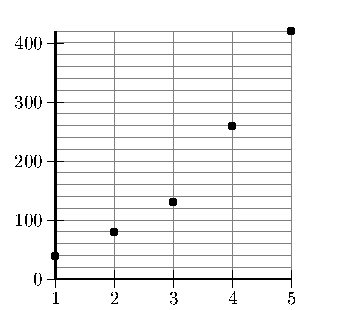
\includegraphics[scale=0.8]{figexo2.pdf}
\end{center}
\item Compléter dans le tableau la ligne indiquant $ z_{i}=\log y_{i} $. \textit{(arrondir à $0,01$ près)}
\item Représenter le nuage de points $ B_{i}(x_{i},z_{i}) $ dans le repère ci-dessous :\\
\begin{center}
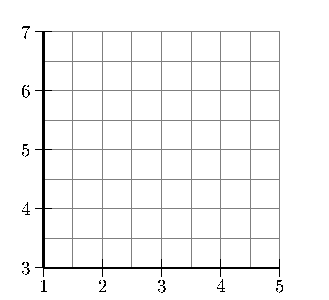
\includegraphics[scale=0.8]{figexo3.pdf}
\end{center}
\item Donner une équation de la droite de régression de $ z $ en $ x $ obtenue par la méthode des moindres carrés et tracer cette droite dans le repère. \textit{($ a $ et $ b $ seront arrondis à $0,001$ près)}
\item En déduire l'expression de $ y $ en fonction de $ x $ en suivant ce modèle. \textit{(on écrira $ y $ sous la forme $ A\times 10^{Bx} $ en arrondissant $ A $ à $ 0,001 $  près)}
\item Selon ce modèle, quel serait le nombre d'abonnés en 2022 ? \textit{(donner le résultat au millier près)}
\end{enumerate}
\end{exocor}

\section{Corrigés}
\begin{corrige}
$\overline{x}=207,8$ \hspace*{0.2cm};\hspace*{0.2cm}$\overline{y}=700$
\end{corrige}

\begin{corrige}
On doit avoir $ \left\lbrace
\begin{array}{l}
\dfrac{8,2+7,4+x+6,1+9}{5}=7,5\\
\dfrac{15+12,1+16,3+y+12}{5}=12,6
\end{array}
\right.$\\
$\Leftrightarrow \left\lbrace
\begin{array}{l}
\dfrac{30,7+x}{5}=7,5\\
\dfrac{55,4+y}{5}=12,6
\end{array}
\right. \Leftrightarrow \left\lbrace
\begin{array}{l}
30,7+x=37,5\\
55,4+y=63
\end{array}
\right.\Leftrightarrow \left\lbrace
\begin{array}{l}
x=6,8\\
y=7,6
\end{array}
\right.$
\end{corrige}

\begin{corrige}
\begin{enumerate}
\item ~\\
\begin{center}
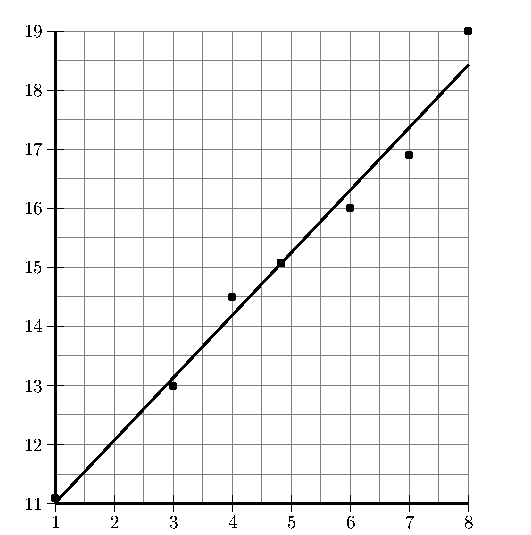
\includegraphics[scale=1]{corr_figure1.pdf} 
\end{center}
\item $\overline{x}=4,83$ \hspace*{0.2cm};\hspace*{0.2cm}$\overline{y}=15,8$
\item $y=1,06x+9,95$
\end{enumerate}
\end{corrige}

\begin{corrige}
\begin{enumerate}
\item $y=0,12x+7,84$
\item Si $x=75$, $y\approx 16,8$
\end{enumerate}
\end{corrige}

\begin{corrige}
\begin{enumerate}
\item ~ \\\begin{tabular}{|c|c|c|c|c|}
\hline Année & 1850 & 1900 & 1950 & 1990 \\ 
\hline Rang de l'année : $ x_{i} $ & 0 & 50 & 100 & 140 \\ 
\hline Teneur en $\mathrm{CO_{2}} $ : $ y_{i} $ & 275 & 290 & 315 & 360 \\ 
\hline $ z_{i}=\log (y_{i}-250) $ & 1,398 & 1,602 & 1,813 & 2,041 \\ 
\hline 
\end{tabular}
\item $z=0,004537x+1,3846$
\item 2050 correspond à $x=200$.\\
On a alors $z \approx 0,004537 \times 200 +1,3846 \Leftrightarrow \log (y-250) \approx 2,292 \Leftrightarrow y-250 \approx 10^{2,292} $\\$\Leftrightarrow y \approx 250+10^{2,292} \approx 446 $
\end{enumerate}
\end{corrige}

\begin{corrige}
\begin{enumerate}
\item Non.
\item ~\\
\begin{center}
\begin{tabular}{|c|c|c|c|c|c|}
\hline Année & 2014 & 2015 & 2016 & 2017 & 2018 \\ 
\hline Rang de l'année $ x_{i} $ & 1 & 2 & 3 & 4 & 5 \\ 
\hline Nombre d'abonnés $ y_{i} $ (en milliers) & 40 & 80 & 130 & 260 & 420 \\ 
\hline $ z_{i}=\log y_{i} $  & 4,602 & 4,903 & 5,114 & 5,415 & 5,623 \\ 
\hline 
\end{tabular} 
\end{center}
\item ~ \\
\begin{center}
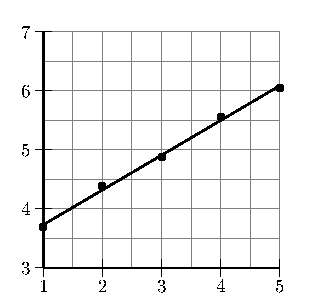
\includegraphics[scale=1]{corr_figure2.pdf} 
\end{center}
\item $z=0,255x+4,365$
\item $\log y=0,255x+4,365 \Leftrightarrow y=10^{0,255x+4,365}=10^{0,255x} \times 10^{4,365}  \approx 23,173 \times 10^{0,255x} $
\item 2022 correspond à $x=9$. \\
On a alors $y \approx 23,173 \times 10^{0,255 \times 9} \approx 4570$ milliers d'abonnés.
\end{enumerate}
\end{corrige}
\end{document}
